% \vspace*{-1cm}
To solve the Ludo problem a GA is applied with single population, generational replacement, 
one point crossover, no elitism and 
standard floating point mutation with a mutation rate of $5\%$.
Here the selection method and crossover rate is determined by testing the different configurations displayed
in table~\ref{tab:configs}.
\vspace*{-0.2cm}
\begin{table}
	\begin{small}
		\begin{center}
			\caption{Selection methods and crossover rates to test}
			\label{tab:configs}
			\begin{tabular}[c]{|l|l|l|l|}
				\hline
				 Selection method/ Crossover rate & $25\%$ & $50\%$ & $75\%$  \\ \hline
				 Tournament                      &  C1      &    C2    & C3 \\ \hline
				 Roulette                        &  C4      &    C5    & C6 \\
				\hline
			\end{tabular}
		\end{center}
	\end{small}
\end{table}
\begin{figure}
		\begin{center}
			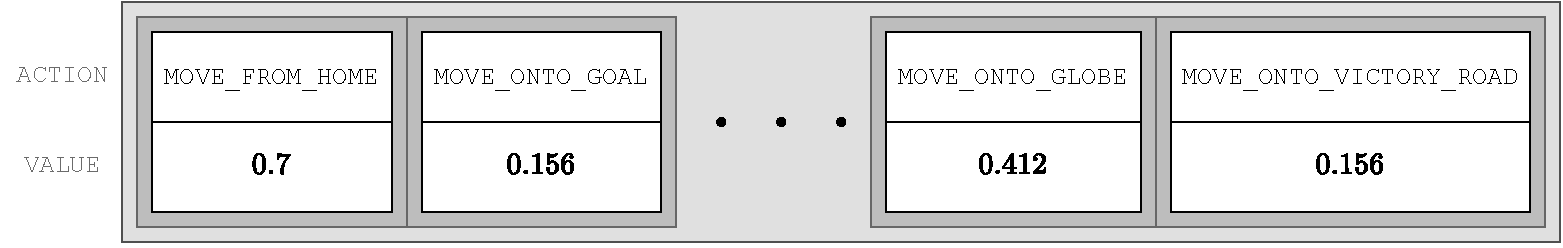
\includegraphics[width=\textwidth]{fig/genome_rep_list.drawio.pdf}
		\end{center}
		\caption{Example of chromosome representation for GA.}
		\label{fig:chromosome_rep}
\end{figure}
The chromosome representation of each player individual is a list of genes in the form of couples, where the 
first element is the enum corresponding to a possible action e.g. \texttt{MOVE\_FROM\_HOME}
while the second element is the value associated with the action. Here actions of greater value
are associated with greater importance. This chromosome representation can be seen exemplified in figure~\ref{fig:chromosome_rep}.
This representation is used due to it containing a great variety of possible actions
during a game, while being compact enough to not contain all possible states.
The standard floating point mutation is performed by having a 5\% probability of
adding a value $\delta\in[-1,1]$ chosen uniformly in the interval.
The goal is thus to determine which actions are better than others, by changing their values such
that the action with the greatest value in a state, generally causes the individual to win more often.
Thus the end result being a ranked list of all actions, from least important action to the most.\par
\begin{table}
	\begin{center}
		\caption{Actions available to the player}
		\label{tab:actions}
		\begin{tabular}[c]{|l|}
			\hline
			Actions \\ \hline
			\texttt{MOVE\_FROM\_HOME} \\
			\texttt{MOVE\_FROM\_HOME\_AND\_KILL} \\
			\texttt{MOVE} \\
			\texttt{MOVE\_ONTO\_STAR} \\
			\texttt{MOVE\_ONTO\_STAR\_AND\_DIE} \\
			\texttt{MOVE\_ONTO\_STAR\_AND\_KILL} \\
			\texttt{MOVE\_ONTO\_GLOBE} \\
			\texttt{MOVE\_ONTO\_GLOBE\_AND\_DIE} \\
			\texttt{MOVE\_ONTO\_ANOTHER\_DIE} \\
			\texttt{MOVE\_ONTO\_ANOTHER\_KILL} \\
			\texttt{MOVE\_ONTO\_VICTORY\_ROAD} \\
			\texttt{MOVE\_ONTO\_GOAL} \\
			\hline
		\end{tabular}
	\end{center}
\end{table} 
In order to include the current state into the decision making, the actions which are impossible
are filtered away when playing the game, such that the agent only is offered the legal actions 
for this particular state. Which ever action has the highest value is then chosen, 
and the game continues.
The different possible actions can be seen in table~\ref{tab:actions}.
One example of such a chromosome can be seen in table~\ref{tab:action-value-paris-example}
with the actions ranked in table~\ref{tab:ranked-action-value-pair-example}. \par
\begin{table}[!htb]
    \begin{minipage}[b]{.5\linewidth}
		\centering
		\caption{Action value pairs example}
		\label{tab:action-value-paris-example}
        \begin{tabular}{|l|l|} \hline
			Action & Value \\ \hline
			\texttt{MOVE\_FROM\_HOME} & 0.785\\
			\texttt{MOVE\_FROM\_HOME\_AND\_KILL} & 0.288\\
			\texttt{MOVE} & 0.512\\
			\texttt{MOVE\_ONTO\_STAR} & 0.339\\
			\texttt{MOVE\_ONTO\_STAR\_AND\_DIE} & 0.023\\
			\texttt{MOVE\_ONTO\_STAR\_AND\_KILL} & 0.591\\
			\texttt{MOVE\_ONTO\_GLOBE} & 0.973\\
			\texttt{MOVE\_ONTO\_GLOBE\_AND\_DIE} & 0.448\\
			\texttt{MOVE\_ONTO\_ANOTHER\_DIE} & 0.915\\
			\texttt{MOVE\_ONTO\_ANOTHER\_KILL} & 0.284\\
			\texttt{MOVE\_ONTO\_VICTORY\_ROAD} & 0.488\\
			\texttt{MOVE\_ONTO\_GOAL} & 0.672\\	\hline
        \end{tabular}
    \end{minipage}%
	\begin{minipage}[b]{.5\linewidth}
      \centering
	  \caption{Ranked action value pairs example}
	  \label{tab:ranked-action-value-pair-example}
	  	\begin{tabular}{|l|l|l|}\hline
			Ranking & Action & Value \\ \hline
			1& \texttt{MOVE\_ONTO\_STAR\_AND\_DIE}  & 0.023\\
			2& \texttt{MOVE\_ONTO\_ANOTHER\_KILL}   & 0.284\\
			3& \texttt{MOVE\_FROM\_HOME\_AND\_KILL} & 0.288\\
			4& \texttt{MOVE\_ONTO\_STAR}            & 0.339\\
			5& \texttt{MOVE\_ONTO\_GLOBE\_AND\_DIE} & 0.448\\
			6& \texttt{MOVE\_ONTO\_VICTORY\_ROAD}   & 0.488\\
			7& \texttt{MOVE}                        & 0.512\\
			8& \texttt{MOVE\_ONTO\_STAR\_AND\_KILL} & 0.591\\
			9& \texttt{MOVE\_ONTO\_GOAL}            & 0.672\\
			10& \texttt{MOVE\_FROM\_HOME}            & 0.785\\
			11& \texttt{MOVE\_ONTO\_ANOTHER\_DIE}    & 0.915\\
			12& \texttt{MOVE\_ONTO\_GLOBE}           & 0.973\\ \hline
		\end{tabular}
	\end{minipage} 
\end{table}
To determine when the algorithm has converged, generally the lack of variation between generations' 
performance can be used, however due to the great variance introduced in Ludo through the dice roll, 
an alternative must be applied. Here a configuration with a crossover rate of $50\%$ and tournament 
selection was made to run until it appeared reasonable to conclude that the algorithm had converged.
The metric chosen to represent a generations performance is the average of all individuals' average
win rates. The number of games played to determine an average win rate for one individual is chosen to be $50$.\par
By inspection the number of generations necessary for convergence was found to be approximately $150$
generations as seen in figure~\ref{fig:convergence}.
\begin{figure}[h]
	\begin{center}
		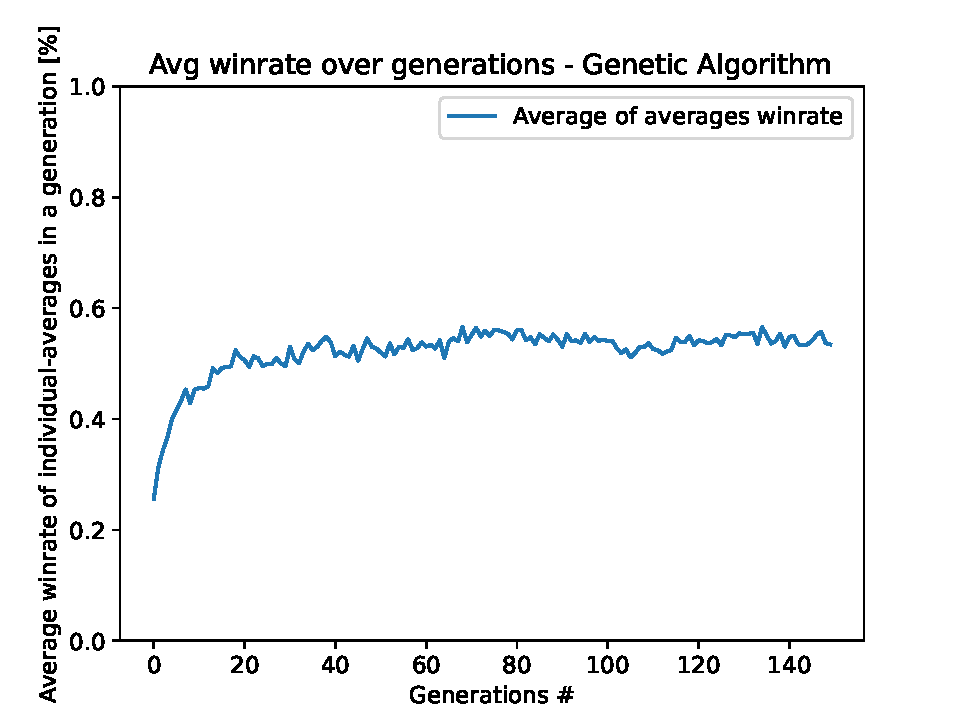
\includegraphics[width=0.7\textwidth]{fig/img_cr_0.5_se_tournament.pdf}
	\end{center}
	\caption{Convergence of GA with a crossover rate of $50\%$ and tournament selection}
	\label{fig:convergence}
\end{figure}
When starting the algorithm $100$ individuals are generated, each with random action values between $0$ and $1$.\par
Each individual is then set to play the before mentioned $50$ games against three dummy players who make 
random moves among the legal
ones presented. By choosing the dummies to be random, an increase in average win rate will indicate 
improvements beyond random variation. \par 
After each individual has played their $50$ games, a fitness score is calculated based on their performance using 
the fitness function in equation (\ref{eq:fitness})
\begin{equation}
	S_{fit} = \overline{WR} \cdot \left( \overline{N}_{kill} + \overline{N}_{tog} \right)
	\label{eq:fitness}
\end{equation}
In this expression $S_{fit} \in \mathbb{R}$ is the fitness score for some particular individual,
$\overline{WR} \in \mathbb{R}$ is the average win rate for said individual after its $50$ games played,
$\overline{N}_{kill}\in\mathbb{R}$ is the number of enemy tokens the player has sent home and
$\overline{N}_{tog} \in \mathbb{R}$ is the average number of tokens the player got to place 
on the goal. \par
This fitness function is formulated such that the win rate scales the other attributes,
making it the dominant trait. The other attributes such as number of tokens on the goal is 
used to encourage a more aggressive play style, while compensated for by the defensive play 
style of killing opponents tokens when possible. By using the win rate as a scaling factor,
an individual with 0 wins will never get to reproduce minimizing the opportunity for undesired fitness exploits. \par
Given (\ref{eq:fitness}), the 6 configurations presented in table~\ref{tab:configs} are
run with the parameters described above. The results can be seen in 
figure~\ref{fig:configs_tested}.
\begin{figure}[h]
	\begin{center}
		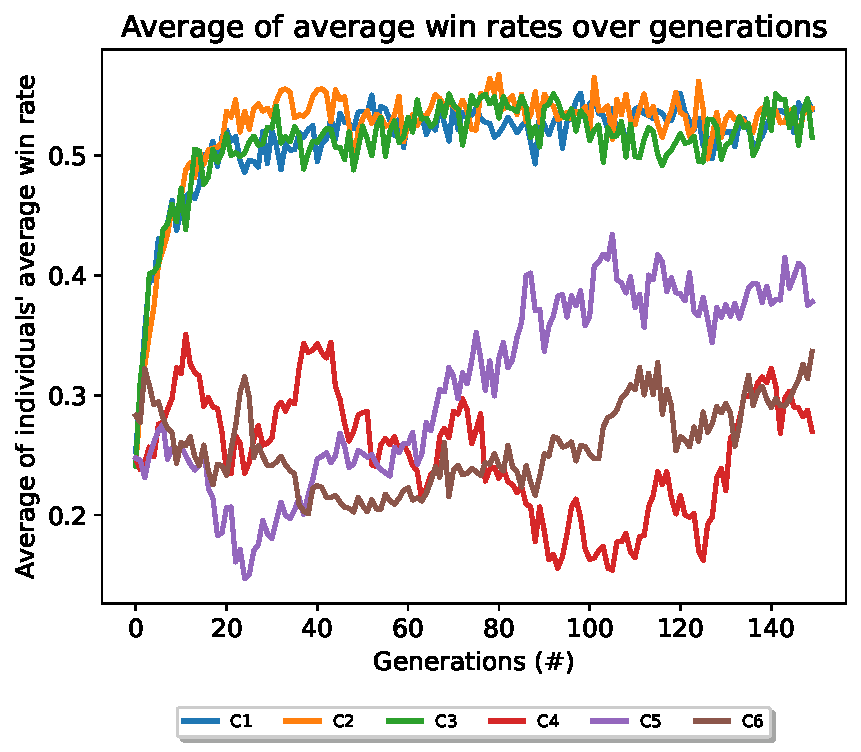
\includegraphics[width=0.7\textwidth]{fig/config_plot.pdf}
	\end{center}
	\caption{Performance of configurations presented in table~\ref{tab:configs}}
	\label{fig:configs_tested}
\end{figure}
Here each data point is the average of average win rates from each 
generation.\par 
To determine if any of the 6 configurations perform statistically best, the 
chromosome with the greatest average win rate from each configuration over all generations are chosen 
as representatives for said configuration. \par
Each of these is set to play $50$ games $1000$ times. These $1000$ win rates are then used to
checked for normality with a Shapiro-Wilk's test, then for equal variance with either a Bartlett
test or a Levene's test depending on the outcome of the previous. A type of ANOVA is then applied
to determine if any of the variables are cause a statistically significant difference. 
This type of ANOVA is dependent on the results from the previous tests.
Finally a 2 sample t-test is applied to determine the best configuration.

\subsection{Comparison of Algorithms}

The best chromosome produced by the algorithm described above will be compared to the 
best chromosome produced in paper \cite*{peter}. The best algorithm produced by this paper 
uses a population size of 128, a cross over rate of 75\%, the bits per crossover is 10\%, 
variant uniform crossover, standard binary mutation, a mutation rate of 1\%, a binary chromosome 
representation and 10\% elitism.

% The algorithm used as comparison to the algorithm of this paper as described above,
% uses a GA algorithm with chromosome representation identical to the one presented 
% in this paper, except the genes are binary. 



% The metric used to determine the performance of any generation, each individual determine its average win rate over 
% the $50$ games played, and each of these averages are applied in a average of averages over the generation.
% By inspection the number of generations necessary for convergence was found to be approximately $150$
% generations as seen in figure~\ref{fig:convergence}. 
% Using this as the baseline for comparison, each configuration in table~\ref{tab:configs} can be compared. \par


	% You do need to describe your representation of the problem and how you encoded it
	% (and why you chose that representation); 

	% you should describe any non-standard choices
	% for operators or procedures; you should state what choices you made for the parameters
	% (e.g. learning rate) and how you chose them (e.g. preliminary test, found in a paper
	% (cited), guessed, etc.); you should describe the tests you conducted to ensure your code
	% works as you claim. Describe what experiments you did.

% You are expected to describe one AI method quite completely (your “own”
% one) and a second one much more briefly. The second one is the one you will be
% comparing against and will have been implemented, and described in detail, by someone
% else (e.g. a partner in your group). Remember to cite and/or acknowledge the source for
% this second method.
% The two methods can be different algorithms, e.g. GA vs. Q-learning, or they can be
% two instances of the same algorithm using different game representations. You are free
% to compare more methods or to try to isolate important factors if you wish, but do not
% exceed the page limit of the paper format.
